\section{Neural Architecture Codesign for Fast Physics Applications}
{{\footnotesize
\begin{description}[labelwidth=5em, labelsep=1em, leftmargin=*, align=left, itemsep=0.3em, parsep=0em]
  \item[date:] 2025-01-09
  \item[version:] TODO
  \item[last\_updated:] 2025-01
  \item[expired:] unknown
  \item[valid:] yes
  \item[valid\_date:] TODO
  \item[url:] \href{https://arxiv.org/abs/2501.05515}{https://arxiv.org/abs/2501.05515}
  \item[doi:] TODO
  \item[domain:] Physics; Materials Science; Particle Physics
  \item[focus:] Automated neural architecture search and hardware-efficient model codesign for fast physics applications
  \item[keywords:]
    - neural architecture search
    - FPGA deployment
    - quantization
    - pruning
    - hls4ml
  \item[summary:] Introduces a two-stage neural architecture codesign (NAC) pipeline combining global and local search,
quantization-aware training, and pruning to design efficient models for fast Bragg peak finding and
jet classification, synthesized for FPGA deployment with hls4ml. Achieves >30x reduction in BOPs
and sub-100 ns inference latency on FPGA.

  \item[licensing:] TODO
  \item[task\_types:]
    - Classification
    - Peak finding
  \item[ai\_capability\_measured:]
    - Hardware-aware model optimization; low-latency inference
  \item[metrics:]
    - Accuracy
    - Latency
    - Resource utilization
  \item[models:]
    - NAC-based BraggNN
    - NAC-optimized Deep Sets (jet)
  \item[ml\_motif:]
    - Real-time, Image/CV
  \item[type:] Framework
  \item[ml\_task:]
    - Supervised Learning
  \item[solutions:] TODO
  \item[notes:] Demonstrated two case studies (materials science, HEP); pipeline and code open-sourced.

  \item[contact.name:] Jason Weitz (UCSD), Nhan Tran (FNAL)
  \item[contact.email:] unknown
  \item[results.links.name:] ChatGPT LLM
  \item[fair.reproducible:] Yes (nac-opt, hls4ml)
  \item[fair.benchmark\_ready:] False
  \item[ratings.software.rating:] 0
  \item[ratings.software.reason:] Not analyzed. 

  \item[ratings.specification.rating:] 10.0
  \item[ratings.specification.reason:] Task is clearly defined (triggering on rare events with sub-10 micros latency); architecture, constraints, and system context (FPGA, Alveo) are well detailed.

  \item[ratings.dataset.rating:] 7.0
  \item[ratings.dataset.reason:] Simulated tracking data from sPHENIX and EIC; internally structured but not yet released in a public FAIR-compliant format.

  \item[ratings.metrics.rating:] 10.0
  \item[ratings.metrics.reason:] Accuracy, latency, and hardware resource utilization (LUTs, DSPs) are clearly defined and used in evaluation.

  \item[ratings.reference\_solution.rating:] 9.0
  \item[ratings.reference\_solution.reason:] Graph-based models (BGN-ST, GarNet) are implemented and tested on real hardware; reproducibility possible with hls4ml but full scripts not bundled.

  \item[ratings.documentation.rating:] 8.0
  \item[ratings.documentation.reason:] Paper is detailed and tool usage (FlowGNN, hls4ml) is described, but repo release and dataset access remain in progress.

  \item[id:] neural\_architecture\_codesign\_for\_fast\_physics\_applications
  \item[Citations:] \cite{weitz2025neuralarchitecturecodesignfast}
  \item[Ratings:]
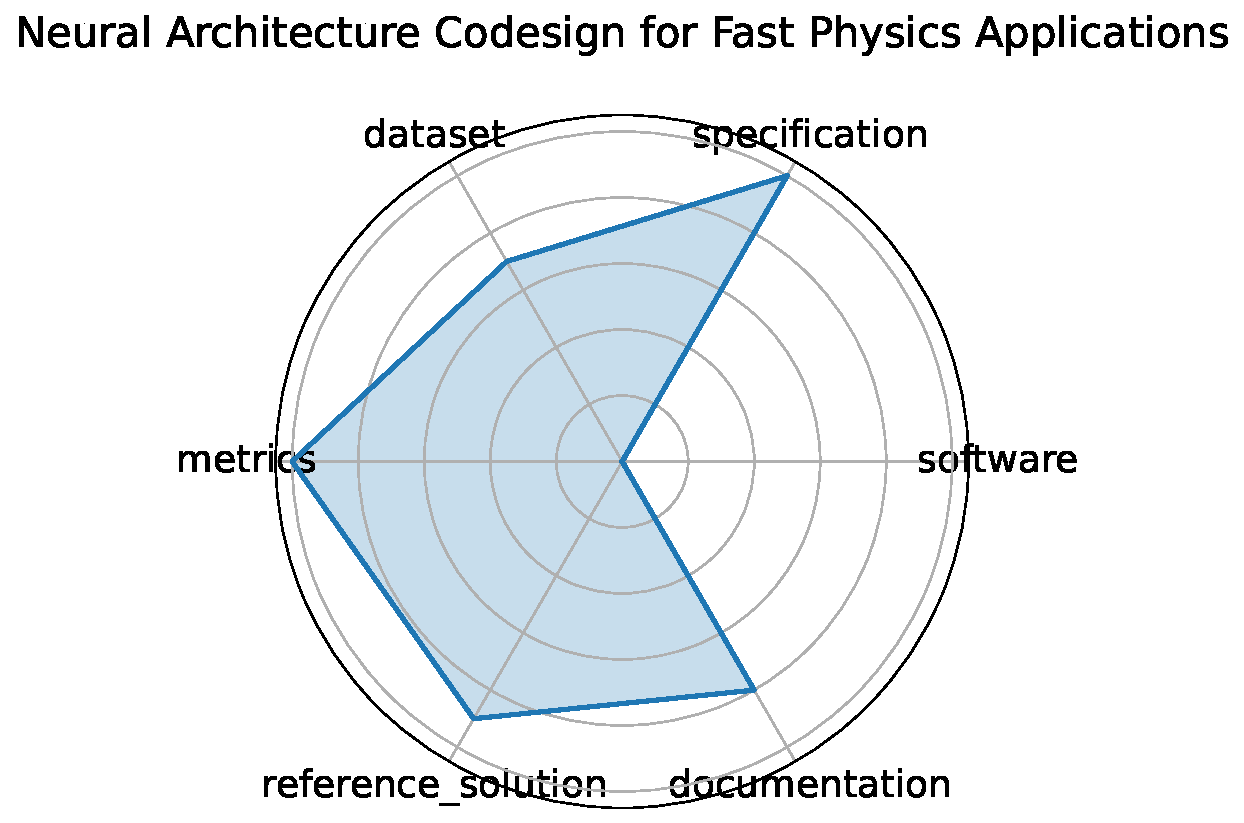
\includegraphics[width=0.2\textwidth]{neural_architecture_codesign_for_fast_physics_applications_radar.pdf}
\end{description}
}}
\clearpage